\chapter{Введение}

Применение нейронных сетей стремительно набирает популярность во многих областях.
Нейросети активно используются широкими массами как в повседневной жизни, так и в
профессиональной деятельности. Их внедряют в голосовых ассистентов, распространенные
среды разработки, системы перевода, а также они выступают в роли самостоятельных
программ для генерации изображений или текста.

Нейронные сети представляют собой сложные вычислительные системы, внутреннее
функционирование которых трудно точно предсказать из-за их ''черного ящика''
(рис. \ref{fig:black_box}) природы. Они принимают на вход набор данных, которые
проходят через множество скрытых слоев, где происходят операции умножения на веса,
сложения и применения нелинейных функций в определенной последовательности.
Эти вычисления в итоге преобразуют входные данные в выходные значения требуемого
формата. В процессе обучения нейросети вычисляется ошибка между полученным выходом
и ожидаемым результатом на обучающих примерах. Затем используются оптимизационные 
алгоритмы для минимизации этой ошибки путем настройки весов внутри сети. 
Таким образом, сеть обучается выполнять желаемую задачу.

\begin{figure}[h]
    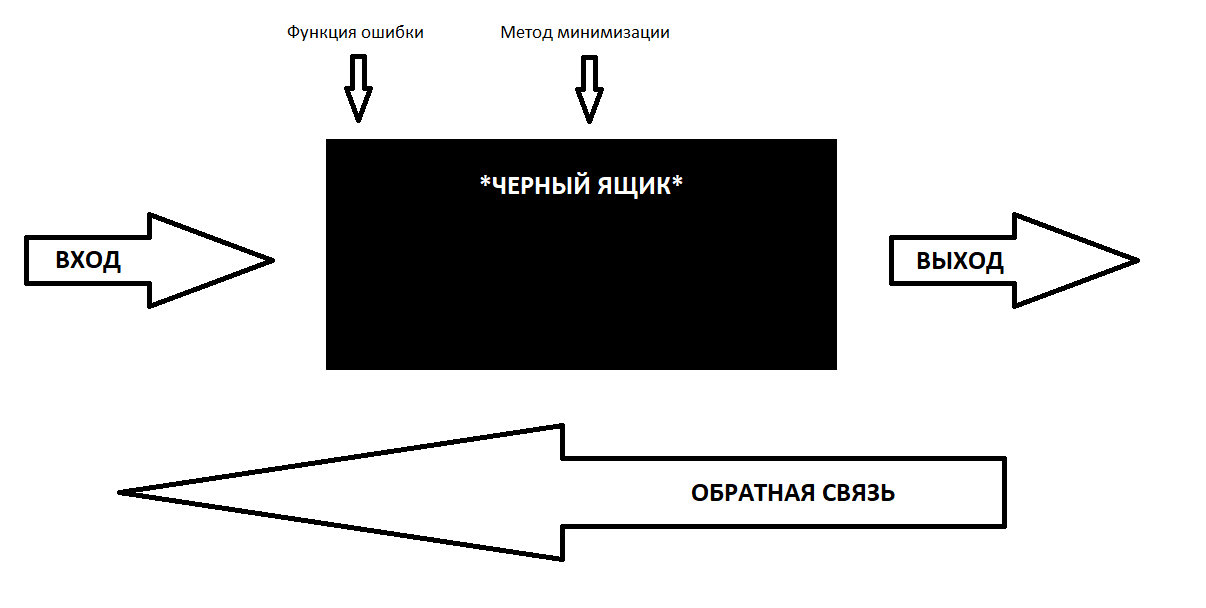
\includegraphics{introdution/black_box.png}
    \caption{Простейшее представление работы нейронной сети}
    \label{fig:black_box}
\end{figure}

Благодаря гибкости функции ошибки, нейронные сети можно использовать для решения
различных уравнений и задач. Функцию ошибки можно задать как невязку между желаемым
решением и выходом нейросети. Этот подход может быть эффективным, поскольку после
однократного обучения нейросеть становится моделью, способной быстро решать целое
семейство однотипных задач. Хотя сам процесс получения предсказаний от обученной
сети также требует вычислительных ресурсов, использование специализированных нейронных
процессоров (NPU) потенциально может ускорить этот процесс без необходимости сложных
оптимизаций и распараллеливания. Таким образом, после начальных затрат на обучение,
нейросеть превращается в эффективный инструмент для быстрого решения множества сходных
задач вычислительного характера.

Для решения широкого круга физических задач можно использовать обученную модель машинного
обучения, которая в качестве входных данных принимает дополнительные безразмерные параметры.
Это позволяет применять одно и то же решение ко многим похожим задачам, варьируя такие
величины, как временной интервал, область, плотность, начальная скорость и т.д., просто
изменяя значения одной или двух дополнительных переменных на входе модели. Точность такого
метода зависит от продолжительности обучения модели, количества скрытых слоев в ее архитектуре
и выбора оптимизатора для обучения. Данный подход очень удобен для получения предварительных
результатов решения физических задач.